\subsection{Features Used in Neural Network}
\label{sec:features}
The features can be devided into two groups, volume density and geometry bias. Volume density captures the local point concentration around a given point, whereas geometry bias accounts for how local surface geometry may distort this measure.

\subsection*{Volume Density Features}
Local volume density can be estimated using either a fixed-radius approach, which counts the number of neighbors within a constant radius for all points, or a fixed-number-of-neighbors approach, which measures the radius required to enclose a fixed number of neighbors around each point. The fixed-radius approach allows the volume density feature to capture information about holes and gaps in the poincloud. In contrast, the fixed-number-of-neighbors approach may obscure such features, as the nearest-neighbor algorithms tend to sample around or beyond holes, reducing their impact on the density estimate (see Figure~\ref{fig:radVSnbh_VD}). 
To ensnure high sensitivity to holes, the fixed-radius approach is preferred. However, a fixed radius is unsuitable across varying point clouds, as it can yield inconsistent neighborhood sizes. Instead, an adaptive radius is defined as the average radius from the fixed-number-of-neighbors approach, based on 20 neighbors. The average radius is used and included as an explicit input feature. This enables the network to interpret local volume density consistently across different scales and sampling resolutions.
The volume density then consists of two features:
\begin{itemize}
    \item \textbf{Average radius}, equal for all points in a single pointcloud 
    \item \textbf{Points inside}, varies for every point
\end{itemize}

\begin{figure}[H]
    \centering
    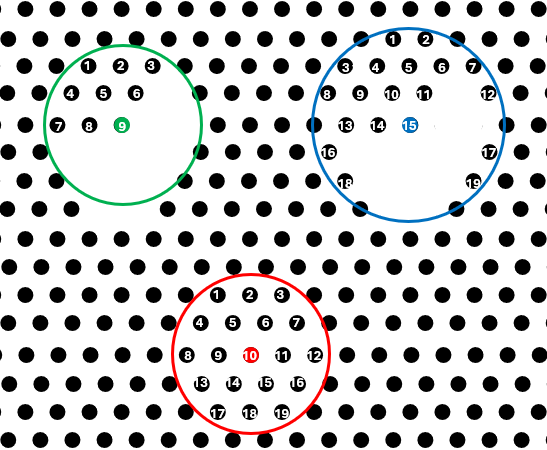
\includegraphics[width=0.4\textwidth]{figures/RadiusVSPoint_based.png}
    \caption{Comparison of volume density estimation using fixed-radius versus fixed-neighborhood methods in the presence of holes.\textbf{Red:} Uniform point distribution with no missing data; both methods yield consistent estimates.\textbf{Green:} Fixed-radius approach near a hole; the radius remains unchanged, but significantly fewer neighbors are included, revealing the presence of a gap.\textbf{Blue:} Fixed-number-of-points approach near a hole; the radius increases slightly to maintain the neighbor count, sampling around the hole reduces sensitivity to the lack of points.}\label{fig:radVSnbh_VD}
\end{figure}

\subsection*{Geometry Bias Features}
Just as a straight line represents the shortest distance between two points, a planar surface is the minimal-area surface that connects any three points. Consequently, a planar region will generally exhibit lower volume density than a curved surface with the same surface density. However, not all geometric influences on volume density are easily measurable. To account for this, multiple geometric features are incorporated to enable the neural network to learn the underlying patterns that define the local geometry bias.
For simplicity, geometry features are computed using the k-nearest neighbors algorithm with a neighborhood size of 20. While this differs slightly from the method used for volume density, the use of the same neighborhood size as the average radius minimizes discrepancies between the feature sets. Five eigenvalue-based features and one gradient-based feature were initially selected to represent the geometry bias. 

The eigenvalue-based features and their formulations are shown in Equation~\ref{eq:eigenvalue_features}, computed using the pyntcloud library[REF]. 

\begin{equation}
\begin{aligned}
    &\lambda_1 \geq \lambda_2 \geq \lambda_3 \geq 0 \\
    \textbf{Curvature} &= \frac{\lambda_3}{\lambda_1 + \lambda_2 + \lambda_3} \\
    \textbf{Linearity} &= \frac{\lambda_1 - \lambda_2}{\lambda_1} \\
    \textbf{Planarity} &= \frac{\lambda_2 - \lambda_3}{\lambda_1} \\
    \textbf{Omnivariance} &= {\lambda_1 + \lambda_2 + \lambda_3}^{1/3} \\
    \textbf{Eigensum} &= \lambda_1 + \lambda_2 + \lambda_3
\end{aligned}
\label{eq:eigenvalue_features}
\end{equation}

where $\lambda_1$, $\lambda_2$ and $\lambda_3$ are the 3 eigenvalues of the covariance matrix for each neighborhood.

For the gradient-based feature, the mean gradient difference was used to quantify local surface variation within a neighborhood. Gradients were computed using the weighted least squares surface fitting approach implemented in the pcdiff library [REF]. Each local surface was fitted to the quadratic form seen in Equation~\ref{eq:surface_fit}:

\begin{equation}
f(x, y) = c_0 + c_1 x + c_2 y + c_3 x^2 + c_4 x y + c_5 y^2
\label{eq:surface_fit}
\end{equation}

The gradient at each point in the neighborhood was then derived analytically with Equation~\ref{eq:grad_vector}.

\begin{equation}
\nabla f(x, y) =
\begin{bmatrix}
\frac{\partial f}{\partial x} \\
\frac{\partial f}{\partial y}
\end{bmatrix}
=
\begin{bmatrix}
c_1 + 2c_3 x + c_4 y \\
c_2 + 2c_5 y + c_4 x
\end{bmatrix}
\label{eq:grad_vector}
\end{equation}

To compute the gradient difference, the L2 norm was applied to the difference between the center points gradient and that of each of its neighbors. The mean of these differences across the neighborhood was used as the final gradient-based feature.

The outputs, for all geometry features, are plotted in Figure~\ref{fig:feature_plot}, for a neighborhood size of 20 points. Omnivariance appears to provide the most substantial information about local geometry. However, both omnivariance and eigensum are proportional to the eigenvalues of the covariance matrix, which scale with the square of the local mesh size. As a result, these features outperformed volume density features during training, but lacked sensitivity to holes and gaps in the data. This led to a model which failed to detect simple voids in the point cloud. Consequently, omnivariance and eigensum were excluded from the final feature set.

\begin{figure*}[t]
    \centering
    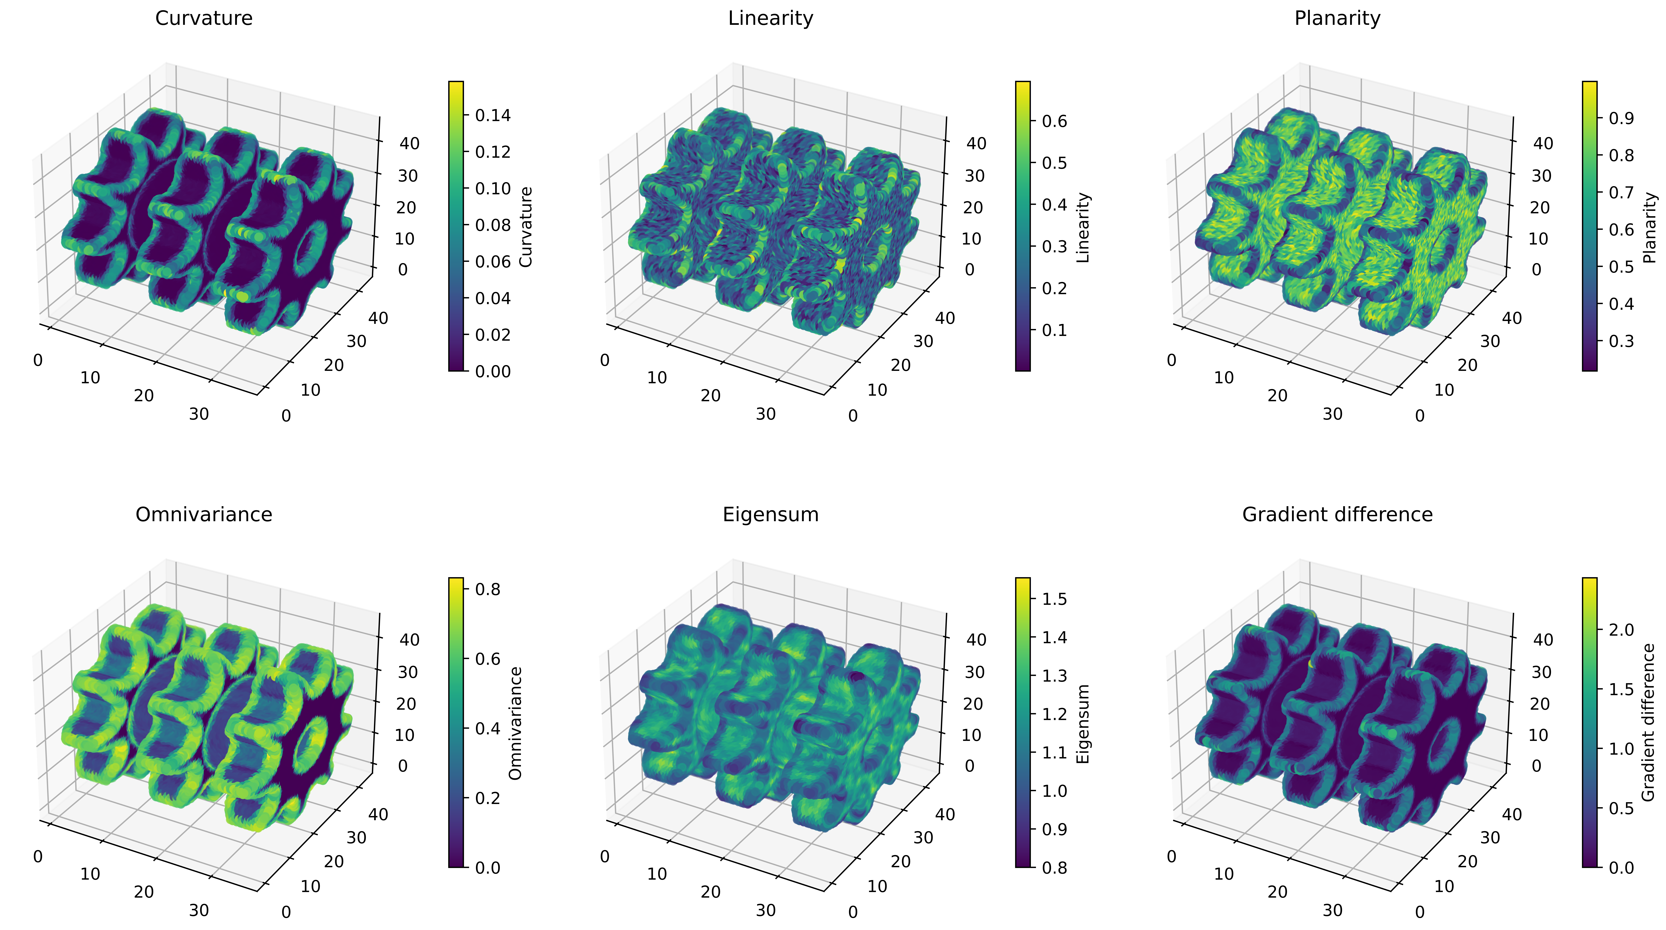
\includegraphics[width=\textwidth]{figures/feature_plots_lowQ.png}
    \caption{Geometry bias features}\label{fig:feature_plot}
\end{figure*}

\subsection*{Final Feature Set}
The features used for training the final model was.
\begin{itemize}
    \item Average Radius
    \item Points inside
    \item Curvature
    \item Linearity
    \item Planarity
    \item Gradient Difference
\end{itemize}